\documentclass[reprint,english,notitlepage]{revtex4-1}  % defines the basic parameters of the document

% if you want a single-column, remove reprint

% allows special characters (including æøå)
\usepackage[utf8]{inputenc}
\usepackage[english]{babel}

%% note that you may need to download some of these packages manually, it depends on your setup.
%% I recommend downloading TeXMaker, because it includes a large library of the most common packages.

\usepackage{physics,amssymb}  % mathematical symbols (physics imports amsmath)
\usepackage{graphicx}         % include graphics such as plots
\graphicspath{{figs/}} %Setting the graphicspath
\numberwithin{equation}{section}
\def\thesection{\arabic{section}}

\usepackage{xcolor}           % set colors
\usepackage{hyperref}         % automagic cross-referencing (this is GODLIKE)
\usepackage{tikz}             % draw figures manually
\usepackage{listings}         % display code
\usepackage{subfigure}        % imports a lot of cool and useful figure commands
\usepackage{pythonhighlight}

% defines the color of hyperref objects
% Blending two colors:  blue!80!black  =  80% blue and 20% black
\hypersetup{ % this is just my personal choice, feel free to change things
    colorlinks,
    linkcolor={red!50!black},
    citecolor={blue!50!black},
    urlcolor={blue!80!black}}

%% Defines the style of the programming listing
%% This is actually my personal template, go ahead and change stuff if you want
\lstset{ %
	inputpath=,
	backgroundcolor=\color{white!88!black},
	basicstyle={\ttfamily\scriptsize},
	commentstyle=\color{magenta},
	language=Python,
	morekeywords={True,False},
	tabsize=4,
	stringstyle=\color{green!55!black},
	frame=single,
	keywordstyle=\color{blue},
	showstringspaces=false,
	columns=fullflexible,
	keepspaces=true}


%% USEFUL LINKS:
%%
%%   UiO LaTeX guides:        https://www.mn.uio.no/ifi/tjenester/it/hjelp/latex/
%%   mathematics:             https://en.wikibooks.org/wiki/LaTeX/Mathematics

%%   PHYSICS !                https://mirror.hmc.edu/ctan/macros/latex/contrib/physics/physics.pdf

%%   the basics of Tikz:       https://en.wikibooks.org/wiki/LaTeX/PGF/TikZ
%%   all the colors!:          https://en.wikibooks.org/wiki/LaTeX/Colors
%%   how to draw tables:       https://en.wikibooks.org/wiki/LaTeX/Tables
%%   code listing styles:      https://en.wikibooks.org/wiki/LaTeX/Source_Code_Listings
%%   \includegraphics          https://en.wikibooks.org/wiki/LaTeX/Importing_Graphics
%%   learn more about figures  https://en.wikibooks.org/wiki/LaTeX/Floats,_Figures_and_Captions
%%   automagic bibliography:   https://en.wikibooks.org/wiki/LaTeX/Bibliography_Management  (this one is kinda difficult the first time)
%%   REVTeX Guide:             http://www.physics.csbsju.edu/370/papers/Journal_Style_Manuals/auguide4-1.pdf
%%
%%   (this document is of class "revtex4-1", the REVTeX Guide explains how the class works)


%% CREATING THE .pdf FILE USING LINUX IN THE TERMINAL
%%
%% [terminal]$ pdflatex template.tex
%%
%% Run the command twice, always.
%% If you want to use \footnote, you need to run these commands (IN THIS SPECIFIC ORDER)
%%
%% [terminal]$ pdflatex template.tex
%% [terminal]$ bibtex template
%% [terminal]$ pdflatex template.tex
%% [terminal]$ pdflatex template.tex
%%
%% Don't ask me why, I don't know.
\newcommand{\TT}{\textsf{T}}
\newcommand{\LL}{\textsf{L}}
\newcommand{\MM}{\textsf{M}}

\begin{document}
\title{AST3220 - Project 3: \\ Inflation without approximation}   % self-explanatory
\author{Candidate nr. 14}
\date{\today}                             % self-explanatory
\noaffiliation                            % ignore this
               % marks the end of the abstract
\maketitle                                % creates the title, author, date & abstract

% the fundamental components of scientific reports:
\section{Problem a)}
Using the convention of represent
As $H_i$ neccesarily has the same dimensions as $H$ it is clear that $h$ must
be dimensionless:
\begin{align}
	[h] = [H] [H_i]^{-1} = 1
\end{align}
The hubble parameter has dimension velocity per distance, which can be written
\begin{align}
	[H] = (\LL \TT^{-1}) \LL^{-1} = \TT^{-1}
\end{align}
so that $\tau$ is dimensionless as well:
\begin{align}
  [\tau] = [H] [t] = \TT^{-1} \TT = 1
\end{align}
Both $\phi$ and the Planck energy has units of energy, making $\psi$ dimensionless
as well:
\begin{align}
	[\psi] = [\phi] [E_p]^{-1} = \MM \LL^2 \TT^{-2} (\MM \LL^2 \TT^{-2})^{-1} = 1
\end{align}
Lastly, we rewrite the potential $v$ using the definiton $E_p^2 = \hbar c^5/G$,
so that
\begin{align}
	v = \frac{\hbar c^3}{H_i^2 E_p^2} = \frac{1}{H_i^2} \frac{G}{c^2}V
\end{align}
Using the definiton of $H_i$, we then see that
\begin{align}
	[v] = [H_i]^{-1} [G c^{-2} V] = [H_i]^{-1}[H_i] = 1
\end{align}
so $v$ is dimensionless as well

\section{Problem b)}
\subsection{Hubble parameter and scale factor}
Using the definitons of the dimensionless variables and applying the chain rule,
we see that
\begin{align}
	\frac{d}{d\tau}\left(\ln \frac{a}{a_i}\right)
				&= \frac{dt}{d\tau}\frac{d}{dt}\left(\ln \frac{a}{a_i}\right) \\
				&= \frac{1}{H_i} \frac{\dot{a}}{a} \\
				&= \frac{H}{H_i} \\
				&= h
\end{align}
\subsection{Continuity equation (name???)}
Similarly we continue using the chain rule to rewrite $\dot{\phi}$,
$\ddot{\phi}$ and $V$' in terms of $\tau$ and $\psi$:
\begin{align}
	\frac{d\phi}{dt} &= \frac{d\tau}{dt}\frac{d\phi}{d\psi}\frac{d\psi}{d\tau}
									 = H_i E_p \frac{d\psi}{d\tau} \\
  \frac{d^2\phi}{dt^2} &= \frac{d\tau}{dt}\frac{d}{d\tau}\frac{d\phi}{dt}
									 = H_i^2 E_p \frac{d^2\psi}{d\tau^2} \\
	\frac{dV}{d\phi} &= \frac{d\psi}{d\phi}\frac{dV}{dv}\frac{dv}{d\psi}
									 = \frac{1}{E_p} \frac{H_i^2 E_p^2}{\hbar c^3} \frac{dv}{d\psi}
\end{align}
Which can be inserted to the (????) equation, giving
\begin{align}
	H_i^2 E_p \frac{d^2\psi}{d\tau^2} + 3H H_i E_p \frac{d\psi}{d\tau}
				+ H_i^2 E_p \frac{dv}{d\psi} = 0
\end{align}
Dividing both sides by $H_i^2 E_p$ and using the definition $h=H/H_i$, this
reduces to
\begin{align}
	\frac{d^2\psi}{d\tau^2} + 3h\frac{d\psi}{d\tau} + \frac{dv}{d\psi} = 0 \label{eq:eom}
\end{align}
\subsubsection{Hubble parameter}
afgasfas
\begin{align}
	h^2 = \frac{8\pi}{3}\left[ \frac{1}{2}\left(\frac{d\psi}{d\tau}\right)^2 + v(\psi)\right] \label{eq:h}
\end{align}
\section{Problem c)}
Read up on this shit

\section{Problem d)}
During slow-roll, the number of remaining e-folds until inflation ends can be
calculated as
\begin{align}
	N(t) &= \frac{8\pi}{E_p^2} \int_{\phi_{\mathrm{end}}}^\phi \frac{V}{V'} d\phi \\
\end{align}
Where we easily find
\begin{align}
	\frac{V}{V'} = \frac{1}{2}\phi
\end{align}
and $\psi_{\mathrm{end}}$ is given by requiring $\epsilon(\phi_{\mathrm{end}})=1$:
\begin{align}
	\epsilon(\phi_{\mathrm{end}}) &= \frac{E_p^2}{16\pi} \left(\frac{V'}{V}\right)^2 \\
											 &= \frac{E_p^2}{4\pi \phi_{\mathrm{end}}^2} \\
											 &= 1 \\
	\Rightarrow \ \ \ \ \phi_{\mathrm{end}} &= \frac{E_p}{\sqrt{4\pi}}
\end{align}
We can then calculate the integral:
\begin{align}
	N(t) &= \frac{8\pi}{E_p^2} \int_{\phi_{\mathrm{end}}}^\phi \frac{1}{2}\phi d\phi \\
					&= \frac{2\pi}{E_p^2} \left(\phi -\frac{E_p^2}{4\pi} \right) \\
					&= \frac{2\pi}{E_p^2} \phi^2 - \frac{1}{2}
\end{align}
By definition, the number of remaining e-folds at the initial time $t=t_i$ is
the total number of e-folds $N_tot$. Evaluating $N(t)$ at $t_i$ and solving for
the initial field value $\phi_i$ we then get:
\begin{align}
	\phi_i = \frac{E_p}{\sqrt{2\pi}}\sqrt{N_{tot} + \frac{1}{2}}
\end{align}
or in terms of the dimensionless field:
\begin{align}
	\psi_i = \sqrt{ \frac{1}{2\pi} \left(N_{tot} + \frac{1}{2} \right) }
\end{align}
Which evaluates to $\psi_i \approx 8.925$ for $500$ e-folds of inflation.

\section{Problem e) \& f)}
To solve the equations of motion of the field, we rename
$\xi = \frac{d\psi}{d\tau}$ so equation \ref{eq:eom} can instead be written as
a set of two first order equations:
\begin{align}
	\frac{d\psi}{d\tau} &= \xi \label{eq:eom_1} \\
	\frac{d\xi}{d\tau}  &= -3h(\xi, \psi) \xi - \frac{d}{d\psi}v(\psi) \label{eq:eom_2}
\end{align}
where $h$ is then given by
\begin{align}
	h^2 = \frac{8\pi}{3}\left[ \frac{1}{2}\xi^2 + v(\psi)\right]
\end{align}
and $v(\psi)$ is given by our choice of potential. Equations \ref{eq:eom_1} and
\ref{eq:eom_2} are then easily solved using a numerical integrator. A plot of
the resulting field $\psi$ plotted against $\tau$ is attached in Figure
(\ref{fig:quad_psi}), along with the slow-roll solution.
\\ \\
With the
solutions $\xi$ and $\psi$ we can easily find $\ln\left(\frac{a}{a_i}\right)$
by numerically evaluating the integral
\begin{align}
	\ln\left(\frac{a}{a_i}\right) &= \int_0^t H dt \\
																&= \int_0^\tau h(\xi, \psi) d\tau
\end{align}
The results are plotted in Figure (\ref{fig:quad_a}), along with the slow-roll
solution
\\ \\
Based on the lectures, we expect the field to decay until it reaches $\psi_{end}$.
When it reaches $\psi_{end}$ it should then start behaving like a damped oscillator
centered around $\psi=0$. This is in agreement with the numerical solution
(Figure \ref{fig:quad_psi}), which starts oscillating at $\tau\approx 1000$.
This is also when the slow-roll approximation starts deviating significantly
from the exact solution, as it instead continues decaying at a constant rate.
\\ \\
This is around the same time the slow-roll approximation for the scale factor
deviates from the exact solution (Figure \ref{fig:quad_a}), as one might expect.
BLABLABLABLA
\begin{figure}[h!]
	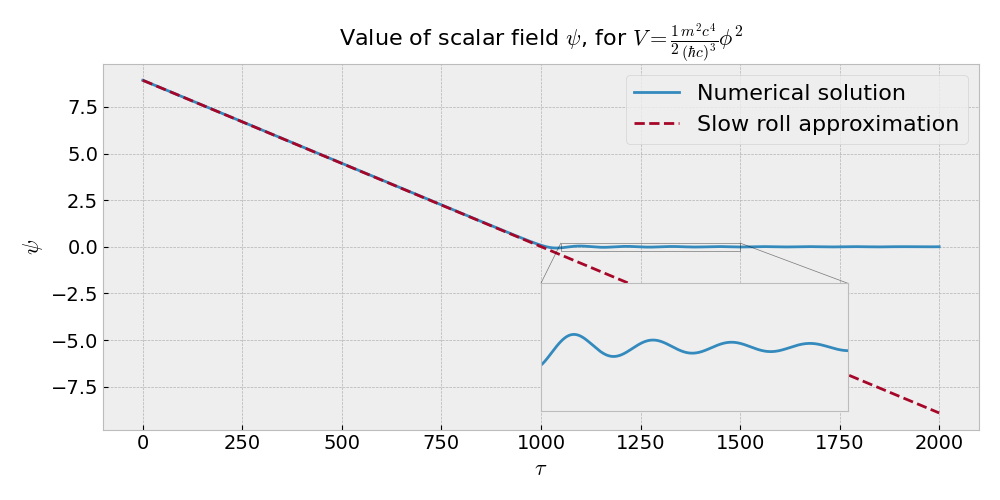
\includegraphics[width=\linewidth]{QuadraticPotential_field-value.png}
	\caption{}
	\label{fig:quad_psi}
\end{figure}

\begin{figure}[h!]
	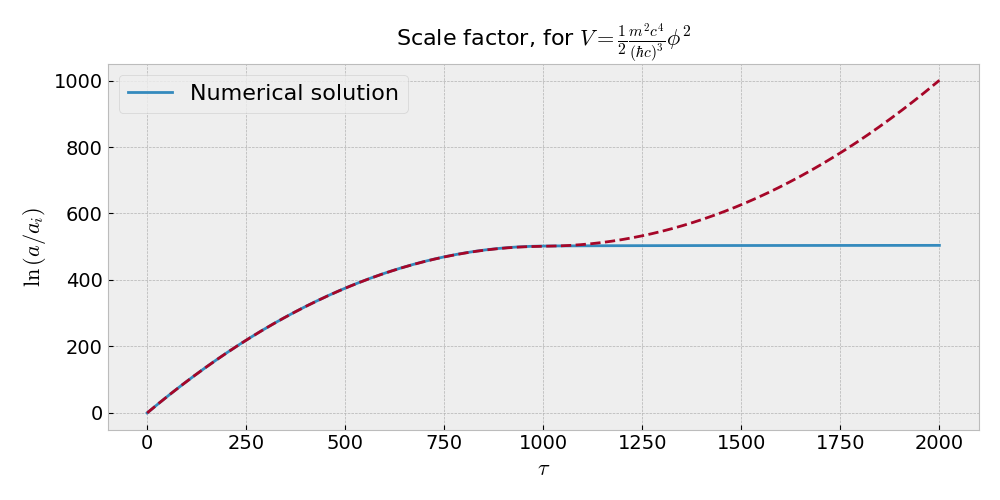
\includegraphics[width=\linewidth]{QuadraticPotential_scale-factor.png}
	\caption{}
	\label{fig:quad_a}
\end{figure}

\section{Problem g)}
\begin{figure}[h!]
	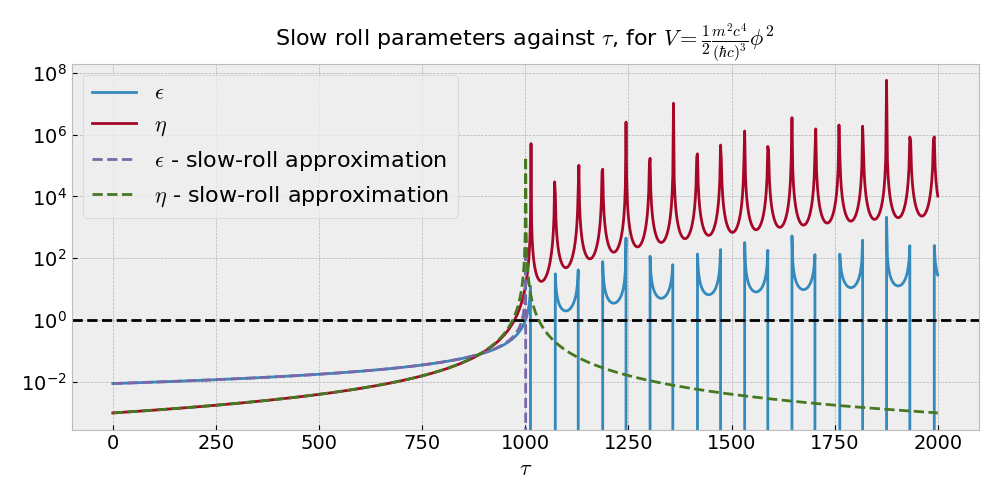
\includegraphics[width=\linewidth]{QuadraticPotential_slowroll-tau.png}
	\caption{}
	\label{}
\end{figure}

\section{Problem h)}
SHOW CALCULATION

\section{Problem i)}
\begin{figure}[h!]
	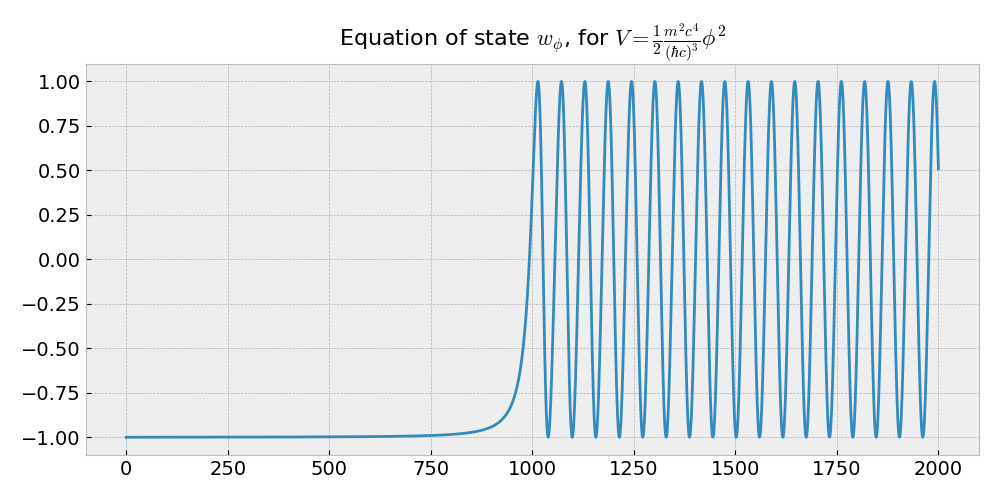
\includegraphics[width=\linewidth]{QuadraticPotential_field-eos.png}
	\caption{}
	\label{}
\end{figure}

\section{Problem j)}
\begin{figure}[h!]
	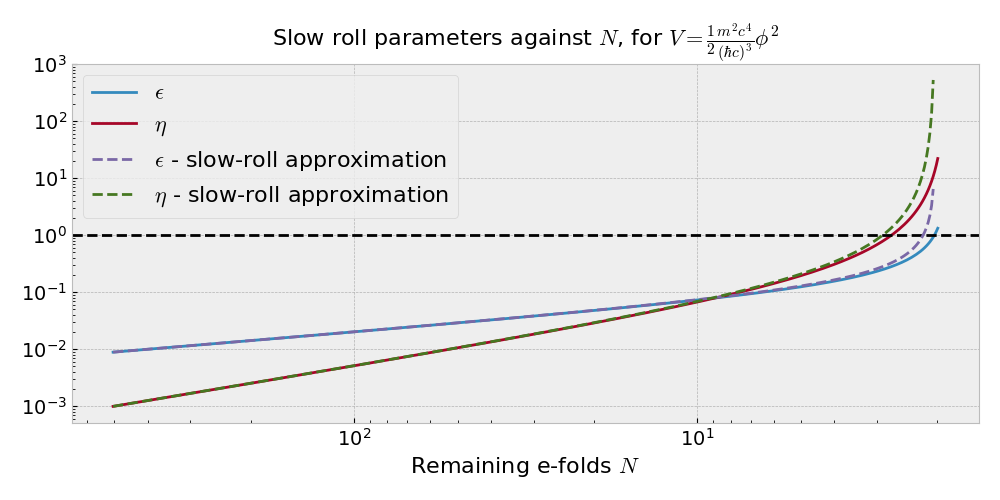
\includegraphics[width=\linewidth]{QuadraticPotential_slowroll-N.png}
	\caption{}
	\label{}
\end{figure}

\section{Problem k)}
\begin{figure}[h!]
	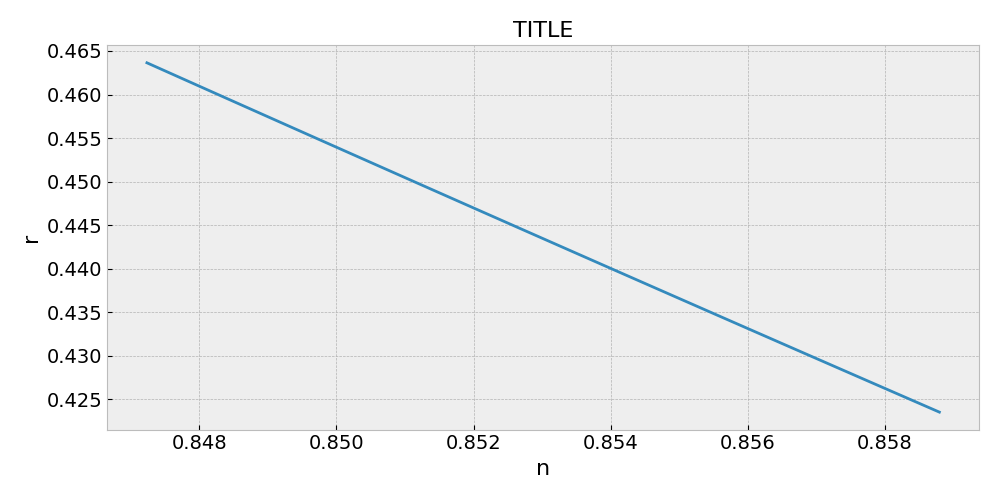
\includegraphics[width=\linewidth]{QuadraticPotential_slowroll-nr.png}
	\caption{}
	\label{}
\end{figure}

\section{Problem l)}
SHOW CALCULATION

\section{Problem m)}
\begin{figure}[h!]
	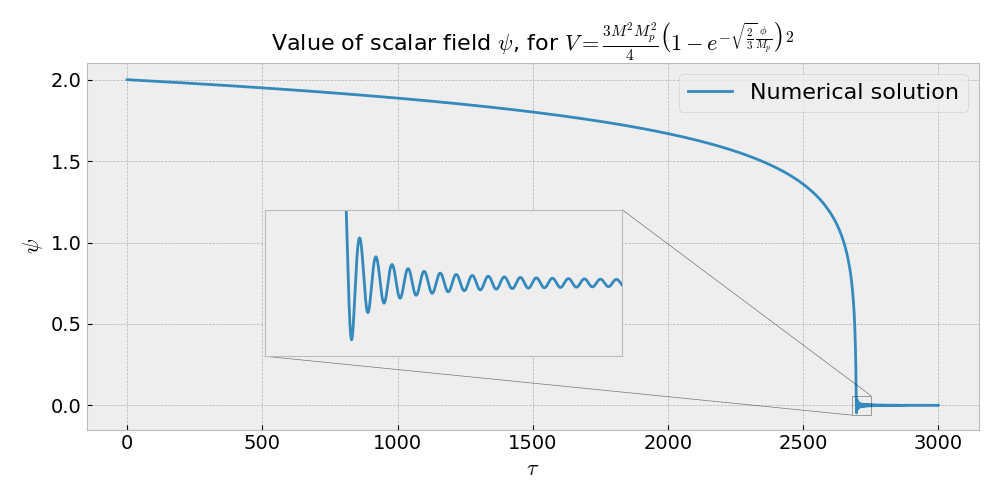
\includegraphics[width=\linewidth]{StarobinskyPotential_field-value.png}
	\caption{}
	\label{}
\end{figure}

\begin{figure}[h!]
	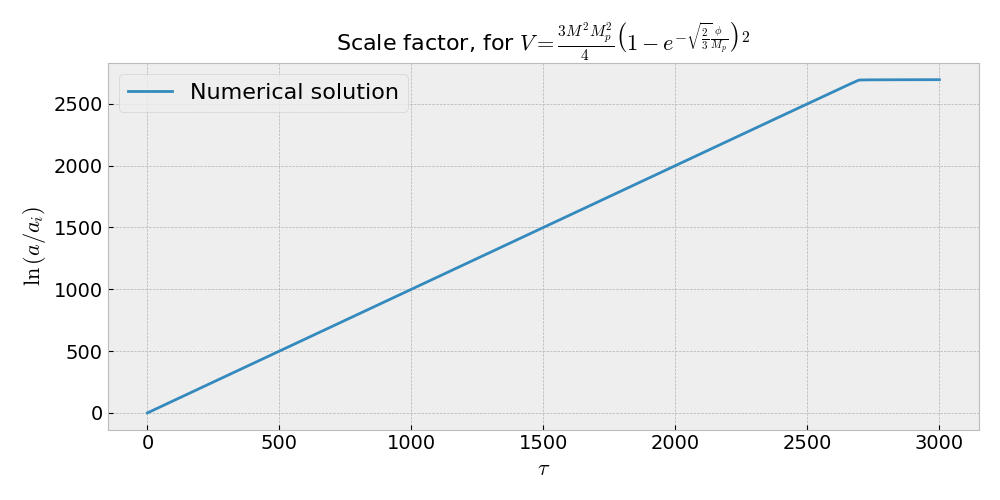
\includegraphics[width=\linewidth]{StarobinskyPotential_scale-factor.png}
	\caption{}
	\label{}
\end{figure}

\section{Problem n)}
\begin{figure}[h!]
	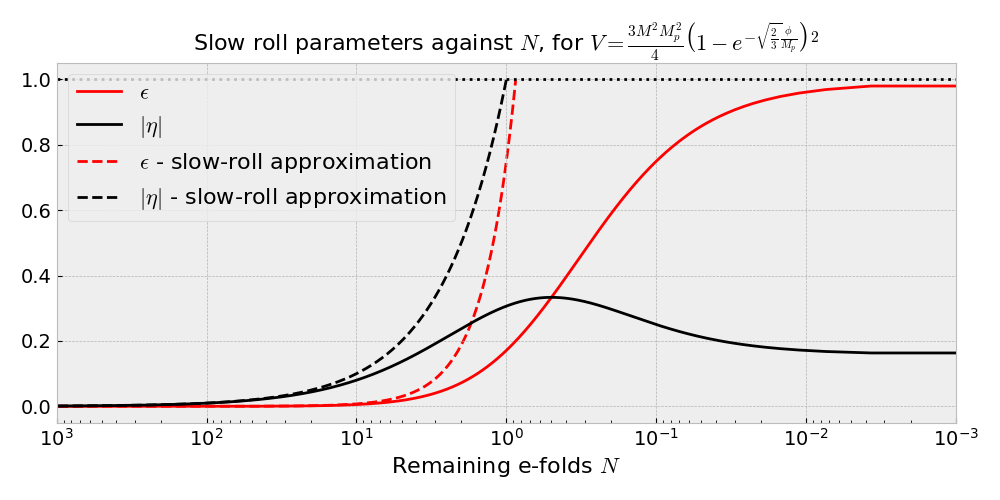
\includegraphics[width=\linewidth]{StarobinskyPotential_slowroll-N.png}
	\caption{}
	\label{}
\end{figure}

\begin{figure}[h!]
	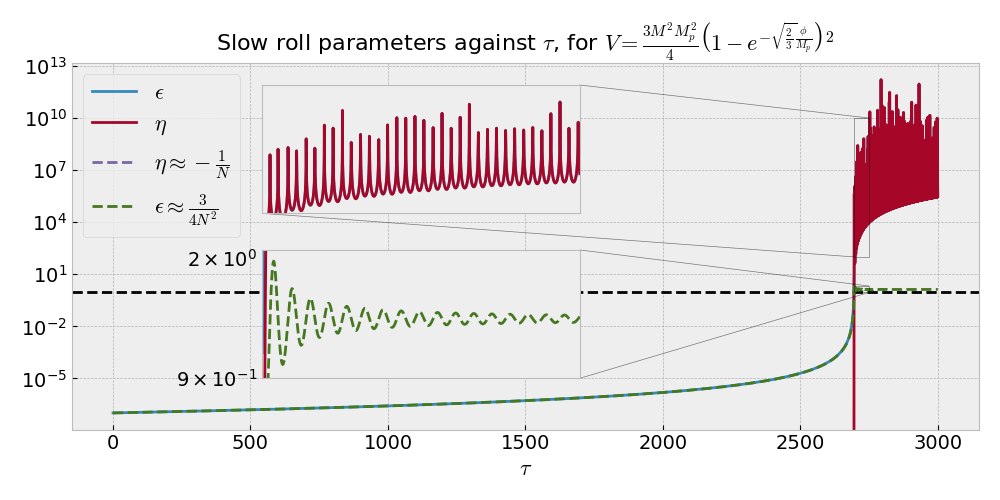
\includegraphics[width=\linewidth]{StarobinskyPotential_slowroll-tau.png}
	\caption{}
	\label{}
\end{figure}

\begin{figure}[h!]
	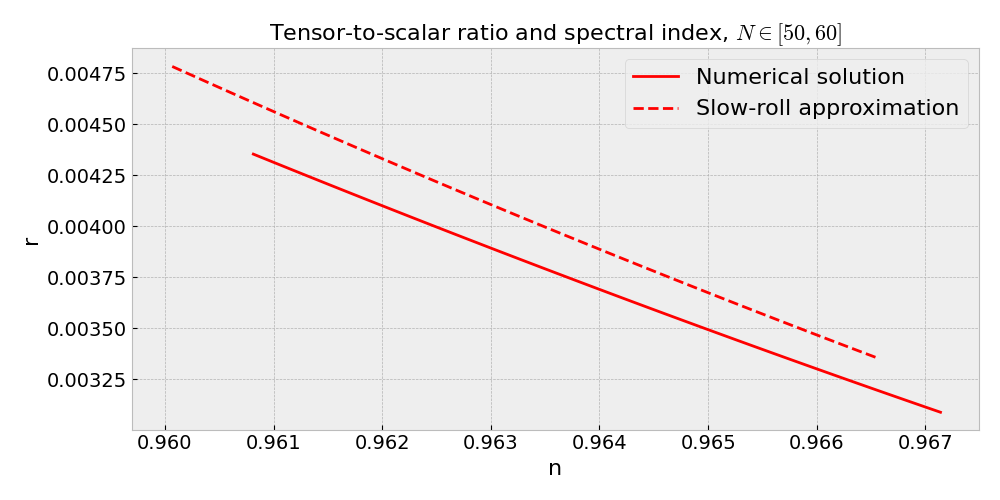
\includegraphics[width=\linewidth]{StarobinskyPotential_slowroll-nr.png}
	\caption{}
	\label{}
\end{figure}

\section{Problem o)}
SHOW CALCULATION

\section{Problem p)}
READ STUFF

\begin{acknowledgments}  % if you disagree with the spelling, blame Americans
I would like thank myself for writing this beautiful document.
\end{acknowledgments}

\end{document}
